\chapter{Editing files with Emacs}\label{emacs-chapter}

FUNNY SOMETHING OR OTHER

\bindex{emacs}
\section{What's Emacs?}

In order to get anything done on a computer, you need a way to put
text into files, and a way to change text that's already in files.  An
{\bf editor} is a program for doing this.  {\tt Emacs} is one of the
most popular editors around---partly because it's very easy for a
complete beginner to get actual work done with it.  (The classic
\unix\ editor, {\tt vi}\ttindex{vi}, is covered in
Appendix~\ref{vi-chapter}.)

To learn {\tt emacs}, you need to find a file of plain text (letters,
numbers, and the like), copy it to your home directory\footnote{For
  instance, {\tt cp /usr/src/linux/README ./README}} (we don't want to
modify the actual file, if it contains important information), and
invoke Emacs on the file:

\begin{screen}
   \begin{tt}
{\tt /home/larry\# emacs README}
   \end{tt}
\end{screen}

(Of course, if you decided to copy {\tt /etc/rc}, {\tt /etc/inittab},
or any other file, substitute that file name for {\tt README}. For
instance, if you {\tt cp /etc/rc \verb+~+/rc}, then {\tt emacs rc}.)

\xwarn ``Invoking'' Emacs can have different effects depending on where
where you do it.  From a plain console displaying only text
characters, Emacs will just take over the whole console.  If you
invoke it from X, Emacs will actually bring up its own window.
I will assume that you are doing it from a text console, but
everything carries over logically into the X Windows version---just
substitute the word ``window'' in the places I've written
``screen''. Also, remeber that you have to move the mouse pointer into
Emacs's window to type in it!

Your screen (or window, if you're using X) should now resemble
Figure~\ref{emacs-shot-1}. Most of the screen contains your text
document, but the last two lines are especially interesting if you're
trying to learn Emacs. The second-to-last line (the one with the long
string of dashes) is called the {\bf mode line}.

\begin{figure}[tbh]\label{emacs-shot-1}
\begin{center}
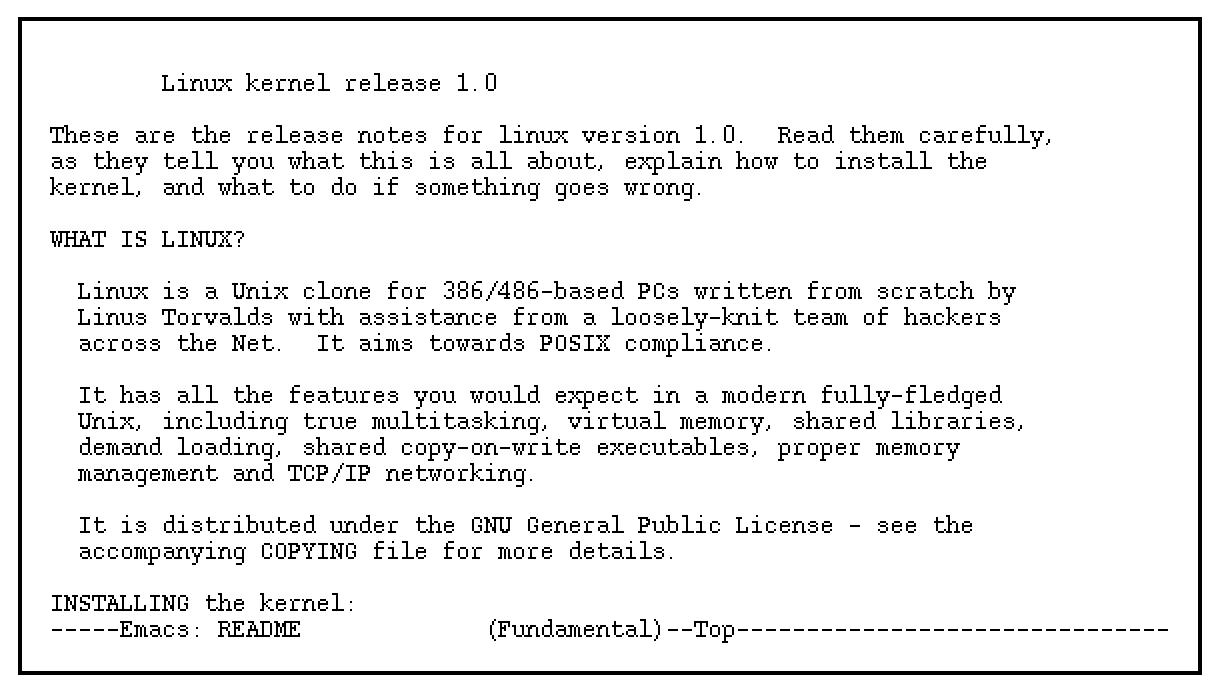
\epsfig{file=ps-files/screen-shot-1.ps, width=5in}
\end{center}
\caption{Emacs was just started with {\tt emacs README}}
\end{figure}

In my mode line, you see ``Top''. It might be ``All'' instead, and
there may be other minor differences. (Many people have the current
time displayed in the mode line.) The line immediately below the mode
line is called the {\bf minibuffer}, or sometimes the {\bf echo area}.
Emacs uses the minibuffer to flash messages at you, and occasionally
uses it to read input from you, when necessary.  In fact, right now
Emacs is telling you ``{\tt For information about the GNU Project and
  its goals, type C-h C-p.}'' Ignore it for now; we won't be making
much use of the minibuffer for a while.

Before you actually change any of the text in the file, you need to
learn how to move around.  The cursor should be at the beginning of
the file, in the upper-left corner of the screen.  To move forward,
type {\tt C-f} (that is, hold down the \key{Control} key while you
press ``f'', for ``forward'').  It will move you forward a character
at a time, and if you hold both keys down, your system's automatic
key-repeat should take effect in a half-second or so.  Notice how when
you get to the end of the line, the cursor automatically moves to the
next line.  {\tt C-b} (for ``backward'') has the opposite behavior.  And,
while we're at it, {\tt C-n} and {\tt C-p} take you to the next and
previous lines, respectively.\footnote{In case you hadn't noticed yet,
  many of Emacs's movement commands consist of combining
  \key{Control} with a single mnemonic letter.}

Using the control keys is usually the quickest way of moving around
when you're editing. The goal of {\tt Emacs} is to keep your hands
over the alpha-numeric keys of the keyboard, where most of your work
gets done. However, if you want to, the arrow keys should also work.

\xwarn In fact, when you're using X, you should be able to position
the mouse pointer and click with the left button to move the cursor
where you want. However, this is very slow---you have to move your
hand all the way to your mouse! Most people who use Emacs primarily
use the keyboard for getting around.

Use {\tt C-p} and {\tt C-b} to get all the way back to the upper-left
corner. Now keep {\tt C-b} held a little longer.  You should
hear an annoying bell sound, and see the message ``{\tt Beginning of
  buffer}'' appear in the minibuffer.  At this point you
might wonder, ``But what is a buffer?''

When Emacs works on a file, it doesn't actually work on the file
itself.  Instead, it copies the contents of the file into a special
Emacs work area called a {\bf buffer}, where you can modify it to your
heart's content.  When you are done working, you tell Emacs to save
the buffer---in other words, to write the buffer's contents into the
corresponding file.  Until you do this, the file remains unchanged,
and the buffer's contents exist only inside of Emacs.

        With that in mind, prepare to insert your first character into
the buffer.  Until now, everything we have done has been
``non-destructive'', so this is a big moment.  You can choose any
character you like, but if you want to do this in style, I suggest
using a nice, solid, capital ``X''.  As you type it, take a look at
the beginning of the mode line at the bottom of the screen.  When you
change the buffer so that its contents are no longer the same as those
of the file on disk, Emacs displays two asterisks at the beginning of
the mode line, to let you know that the buffer has been modified:

\begin{screen}
   \begin{verbatim}
--**-Emacs: some_file.txt           (Fundamental)--Top------------------------
\end{verbatim}
\end{screen}

        These two asterisks are displayed as soon as you modify the
buffer, and remain visible until you save the buffer.  You can save
the buffer multiple times during an editing session---the command to
do so is just {\tt C-x~C-s} (hold down \key{Control} and hit ``x''
and ``s'' while it's down\ldots okay, so you probably already figured
that out!).  It's deliberately easy to type, because saving your
buffers is something best done early and often.

I'm going to list a few more commands now, along with the ones you've
learned already, and you can practice them however you like.  I'd
suggest becoming familiar with them before going any further:

\begin{tabular}{ll}
{\bf {\tt C-f}}       & Move forward one character. \\
{\bf {\tt C-b}}       & Move backward one character. \\
{\bf {\tt C-n}}       & Go to next line. \\
{\bf {\tt C-p}}       & Go to previous line. \\
{\bf {\tt C-a}}       & Go to beginning of line. \\
{\bf {\tt C-e}}       & Go to end of line. \\
{\bf {\tt C-v}}       & Go to next page/screenful of text. \\
{\bf {\tt C-l}}       & Redraw the screen, with current line in center. \\
{\bf {\tt C-d}}       & Delete this character (practice this one). \\
{\bf {\tt C-k}}       & Delete text from here to end of line. \\
{\bf {\tt C-x C-s}}   & Save the buffer in its corresponding file. \\
\key{Backspace}       & Delete preceding character (the one you just typed). \\
\end{tabular}

\section{Getting Started Quickly in X}

\xwarn If all you're interesting in is editing a few files quickly, an
X user doesn't have to go much further beyond the menus at the top of
the screen: 

\begin{center}
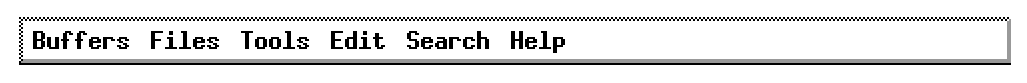
\epsfig{file=ps-files/screen-shot-2.ps,width=\textwidth}
\end{center}

These menus are not available in text mode.

When you first start Emacs, there will be four menus at the top of the
screen: {\sf Buffers}, {\sf File}, {\sf Edit}, and {\sf Help}. To use
a menu, simply move the mouse pointer over the name (like {\sf File},
click and hold down on the left button. Then, move the pointer to the
action you want and release the mouse button. If you change your mind,
move the mouse pointer away from the menu and release the button.

The {\sf Buffers} menu lists the different files you've been editing
in this incarnation of Emacs.The {\sf File} menu shows a bunch of
commands for loading and saving files---many of them will be described
later. The {\sf Edit} menu displays some commands for editing one
buffer, and the {\sf Help} menu should hopefully give on-line
documentation.

You'll notice keyboard equivalents are listed next to the choices in
the menu. Since, in the long run, they'll be quicker, you might want
to learn them. Also, for better or for worse, most of Emacs's
functionality is {\em only\/} available through the keyboard---you
might want to read the rest of this chapter.

\section{Editing Many Files at Once}

Emacs can work on more than one file at a time.  In fact, the only
limit on how many buffers your Emacs can contain is the actual amount
of memory available on the machine. The command to bring a new file
into an Emacs buffer is {\tt C-x~C-f}.  When you type it, you will be
prompted for a filename in the minibuffer:

\begin{screen}
   \begin{verbatim}
Find file: ~/
   \end{verbatim}
\end{screen}

        The syntax here is the same one used to specify files from the
shell prompt; slashes represent subdirectories, \verb+~+means your
home directory.  You also get {\bf filename completion}, meaning
that if you've typed enough of a filename at the prompt to identify
the file uniquely, you can just hit \key{Tab} to complete it (or to
show possible completions, if there are more than one).  \key{Space}
also has a role in filename completion in the minibuffer, similar to
\key{Tab}, but I'll let you experiment to find out how the two differ.
% translation: I know they're different, but I can never figure out how!
Once you have the full filename in the minibuffer, hit \key{Return},
and Emacs will bring up a buffer displaying that file.  In Emacs, this
process is known as {\bf finding} a file.  Go ahead and find some
other unimportant text file now, and bring it into Emacs (do this from
our original buffer {\tt some\_file.txt}).  Now you have a new buffer;
I'll pretend it's called {\tt another\_file.txt}, since I can't see
your mode line.

        Your original buffer seems to have disappeared---you're
probably wondering where it went.  It's still inside Emacs, and you
can switch back to it with {\tt C-x~b}.  When you type this, you will
see that the minibuffer prompts you for a buffer to switch to, and it
names a default.  The default is the buffer you'd get if you just hit
\key{Return} at the prompt, without typing a buffer name.  The default
buffer to switch to is always the one most recently left, so that when
you are doing a lot of work between two buffers, {\tt C-x~b} always
defaults to the ``other'' buffer (which saves you from having to type
the buffer name).  Even if the default buffer is the one you want,
however, you should try typing in its name anyway.

        Notice that you get the same sort of completion you got when
finding a file: hitting \key{Tab} completes as much of a buffer name
as it can, and so on.  Whenever you are being prompted for something
in the minibuffer, it's a good idea to see if Emacs is doing
completion.  Taking advantage of completion whenever it's offered will
save you a lot of typing.  Emacs usually does completion when you are
choosing one item out of some predefined list.

Everything you learned about moving around and editing text in the
first buffer applies to the new one.  Go ahead and change some text in
the new buffer, but don't save it (i.e.\ don't type {\tt C-x~C-s}).
Let's assume that you want to discard your changes without saving them
in the file.  The command for that is {\tt C-x~k}, which ``kills'' the
buffer.  Type it now.  First you will be asked which buffer to kill,
but the default is the current buffer, and that's almost always the
one you want to kill, so just hit \key{Return}.  Then you will be
asked if you {\em really\/} want to kill the buffer---Emacs always
checks before killing a buffer that has unsaved changes in it.  Just
type ``yes'' and hit \key{Return}, if you want to kill it.

        Go ahead and practice loading in files, modifying them, saving
them, and killing their buffers.  Make sure you don't modify any
important system files in a way that will cause trouble\footnote{If
you are not the ``root'' user on the machine, you shouldn't be able to
hurt the system anyway, but be careful just the same.}, of course, but
do try to have at least five buffers open at once, so you can get the
hang of switching between them.

\section{Ending an Editing Session}

When you are done with your work in Emacs, make sure that all buffers
are saved that should be saved, and exit Emacs with {\tt C-x~C-c}.
Sometimes {\tt C-x~C-c} will ask you a question or two in the
minibuffer before it lets you leave---don't be alarmed, just answer
them in the obvious ways.  If you think that you might be returning to
Emacs later, don't use {\tt C-x~C-c} at all; use {\tt C-z}, which will
suspend Emacs.  You can return to it with the shell command ``{\tt
  fg}'' later. This is more efficient than stopping and starting Emacs
multiple times, especially if you have edit the same files again
later.

\xwarn Under X, hitting {\tt C-z} will merely iconize the window. See
the section on iconization in Chapter~\ref{x-chapter}. This gives you
two ways of iconizing Emacs---the normal way your window manager
offers, and {\tt C-z}. Remember, when you iconize, a simply {\tt fg}
won't bring the window back---you'll have to use your window manager.

\section{The Meta Key}

You've already learned about one ``modifier key'' in Emacs, the
\key{Control} key.  There is a second one, called the {\bf Meta}
key, which is used almost as frequently.  However, not all keyboards
have their Meta key in the same place, and some don't have one at all.
The first thing you need to do is find where your Meta key is located.
Chances are, your keyboard's \key{Alt} keys are also Meta keys, if
you are using an IBM PC or other another keyboard that has an
\key{Alt} key.

        The way to test this is to hold down a key that you think
might be a Meta key and type ``x''.  If you see a little prompt appear
in the minibuffer (like this: {\tt M-x}) then you've found it.  To get
rid of the prompt and go back to your Emacs buffer, type {\tt C-g}.

If you didn't get a prompt, then there is still one solution.  You can
use the \key{Escape} key as a Meta key.  But instead of holding it
down while you type the next letter, you have to tap it and release it
quickly, and {\em then\/} type the letter.  This method will work
whether or not you have a real Meta key, so it's the safest way to go.
Try tapping \key{Escape} and then typing ``x'' now.  You should get
that tiny prompt again.  Just use {\tt C-g} to make it go away.  {\tt
  C-g}\index{emacs!interrupting} is the general way in Emacs to quit
out of something you don't mean to be in.  It usually beeps annoyingly
at you to let you know that you have interrupted something, but that's
fine, since that's what you intended to do if you typed {\tt
  C-g}\/!\footnote{Occasionally, even one {\tt C-g} isn't enough to
  persuade Emacs that you really wanted to interrupt what you're
  doing. Just keep at it, and Emacs will usually return to a saner
  mode.}

         The notation {\tt M-x} is analogous to {\tt C-x} (substitute
any character for ``{\tt x}'').  If you have found a real Meta key,
use that, otherwise just use the \key{Escape} key.  I will simply
write {\tt M-x} and you'll have to use your own Meta key.

\section{Cutting, Pasting, Killing and Yanking}
        
Emacs, like any good editor, allows you to cut and paste blocks of
text.  In order to do this, you need a way to define the start and end
of the block.  In Emacs, you do this by setting two locations in the
buffer, known as {\bf mark}\index{emacs!mark} and {\bf
  point}\index{emacs!point}.  To set the mark, go to the place you
want your block to begin and type {\tt C-SPC} (``{\tt SPC}'' means
\key{Space}, of course).  You should see the message ``Mark set''
appear in the minibuffer.\footnote{On some terminals, {\tt C-SPC} doesn't
  work.  For these machines, you must use {\tt C-@}.} The mark has now
been set at that place.  There will be no special highlighting
indicating that fact, but you know where you put it, and that's all
that matters.

What about {\bf point}?  Well, it turns out that you've been setting
point every time you move the cursor, because ``point'' just refers to
your current location in the buffer.  In formal terms, point is the
spot where text would be inserted if you were to type something.  By
setting the mark, and then moving to the end of the block of text, you
have actually defined a block of text.  This block is known as the
{\bf region}\index{emacs!region}.  The region always means the area
between mark and point.

Merely defining the region does not make it available for pasting.
You have to tell Emacs to copy it in order to be able to paste it.  To
copy the region, make sure that mark and point are set correctly, and
type {\tt M-w}.  It has now been recorded by Emacs.  In order to paste
it somewhere else, just go there and type {\tt C-y}.  This is known as
{\bf yanking}\index{emacs!yanking} the text into the buffer.

If you want to actually move the text of the region to somewhere else,
type {\tt C-w} instead of {\tt M-w}.  This will {\bf
  kill}\index{emacs!kill} the region---all the text inside it will
disappear.  In fact, it has been saved in the same way as if you had
used {\tt M-w}.  You can yank it back out with {\tt C-y}, as always.
The place Emacs saves all this text is known as the {\bf kill-ring}.
Some editors call it the ``clipboard'' or the ``paste buffer''.

        There's another way to do cutting and pasting: whenever you
use {\tt C-k} to kill to the end of a line, the killed text is saved
in the kill-ring.  If you kill more than one line in a row, they are
all saved in the kill-ring together, so that the next yank will paste
in all the lines at once.  Because of this feature, it is often faster
to use repeated {\tt C-k}'s to kill some text than it is to explicitly
set mark and point and use {\tt C-w}.  However, either way will work.
It's really a matter of personal preference how you do it.

\section{Searching and Replacing}

There are several ways to search for text in Emacs.  Many of them are
rather complex, and not worth going into here.  The easiest and most
entertaining way is to use {\bf isearch}\bindex{emacs!searching}.
``Isearch'' stands for ``incremental search''.  Suppose you want to
search for the string ``gadfly'' in the following buffer:

\begin{quote}
   \begin{tt}
        I was growing afraid that we would run out of gasoline, when
my passenger exclaimed ``Gadzooks!  There's a gadfly in here!''.
   \end{tt}
\end{quote}

You would move to the beginning of the buffer, or at least to some
point that you know is before the first occurence of the goal word,
``gadfly'', and type {\tt C-s}.  That puts you in isearch mode.  Now
start typing the word you are searching for, ``gadfly''.  But as soon
as you type the ``g'', you see that Emacs has jumped you to the first
occurence of ``g'' in the buffer.  If the above quote is the entire
contents of the buffer, then that would be the first ``g'' of the word
``growing''.  Now type the ``a'' of ``gadfly'', and Emacs leaps over
to ``gasoline'', which contains the first occurence of a ``ga''.  The
``d'' gets you to gadzooks, and finally, ``f'' gets you to ``gadfly'',
without your having had to type the entire word.

        What you are doing in an isearch is defining a string to
search for.  Each time you add a character to the end of the string,
the number of matches is reduced, until eventually you have entered
enough to define the string uniquely.  Once you have found the match
you are looking for, you can exit the search with \key{Return} or any
of the normal movement commands.  If you think the string you're
looking for is behind you in the buffer, then you should use {\tt
C-r}, which does an isearch backwards.

        If you encounter a match, but it's not the one you were
looking for, then hit {\tt C-s} again while still in the search.  This
will move you forward to the next complete match, each time you hit
it.  If there is no next match, it will say that the search failed,
but if you press {\tt C-s} again at that point, the search will wrap
around from the beginning of the buffer.  The reverse holds true for
{\tt C-r} --- it wraps around the end of the buffer.

        Try bringing up a buffer of plain English text and doing and
isearch for the string ``{\tt the}''.  First you'd type in as much as
you wanted, then use repeated {\tt C-s}'s to go to all instances of
it.  Notice that it will match words like ``{\tt them}'' as well,
since that also contains the substring ``{\tt the}''.  To search only
for ``{\tt the}'', you'd have to do add a space to the end of your
search string.  You can add new characters to the string at any point
in the search, even after you've hit {\tt C-s} repeatedly to find the
next matches.  You can also use \key{Backspace} or \key{Delete} to
remove characters from the search string at any point in the search,
and hitting \key{Return} exits the search, leaving you at the last
match.

        Emacs also allows you to replace all instances of a string
with some new string---this is known as {\bf query-replace}.  To
invoke it, type {\tt query-replace} and hit \key{Return}.
Completion is done on the command name, so once you have typed
``query-re'', you can just hit \key{Tab} to finish it.  Say you wish
to replace all instances of ``gadfly'' with ``housefly''.  At the
``{\tt Query replace:\, }'' prompt, type ``gadfly'', and hit
\key{Return}.  Then you will be prompted again, and you should enter
``housefly''.  Emacs will then step through the buffer, stopping at
every instance of the word ``gadfly'', and asking if you want to
replace it.  Just hit ``{\tt y}'' or ``{\tt n}'' at each instance, for
``Yes'' or ``No'', until it finishes.  If this doesn't make sense as
you read it, then try it out.
\eindex{emacs!searching}

\section{What's Really Going On Here?}

        Actually, all these {\bf keybindings} you have been learning
are shortcuts to Emacs functions.  For example, {\tt C-p} is a short
way of telling Emacs to execute the internal function {\tt
previous-line}.  However, all these internal functions can be called
by name, using {\tt M-x}.  If you forgot that {\tt previous-line} is
bound to {\tt C-p}, you could just type {\tt M-x previous-line}
\key{Return}, and it would move you up one line.  Try this now, to
understand how {\tt M-x previous-line} and {\tt C-p} are really the
same thing.

        The designer of Emacs started from the ground up, first
defining a whole lot of internal functions, and then giving
keybindings to the most commonly-used ones.  Sometimes it's easier
just to call a function explicitly with {\tt M-x} than to remember
what key it's bound to.  The function {\tt query-replace}, for
example, is bound to {\tt M-\%} in some versions of Emacs.  But who
can remember such an odd keybinding?  Unless you use query-replace
extremely often, it's easier just to call it with {\tt M-x}.

        Most of the keys you type are letters, meant to be inserted
into the text of the buffer.  So each of those keys is {\bf bound} to
the function {\tt self-insert-command}, which does nothing but insert
that letter into the buffer.  Combinations that use the \key{Control}
key with a letter are generally bound to functions that do other
things, like moving you around.  For example, {\tt C-v} is bound to a
function called {\tt scroll-up}, which scrolls the buffer up by one
screenful (meaning that your position in the buffer moves {\em
down\/}, of course).

        If you ever actually wanted to insert a Control character into
the buffer, then, how would you do it?  After all, the Control
characters are {\tt ASCII} characters, although rarely used, and you
might want them in a file.  There is a way to prevent Control
characters from being interpreted as commands by Emacs.  The key {\tt
C-q}\footnote{We call {\tt C-q} a ``key'', even though it is produced
by holding down \key{Control} and pressing ``q'', because it is a
single {\tt ASCII} character.} is bound to a special function named
{\tt quoted-insert}.  All {\tt quoted-insert} does is read the next
key and insert it literally into the buffer, without trying to
interpret it as a command.  This is how you can put Control characters
into your files using Emacs.  Naturally, the way to insert a C-q is to
press {\tt C-q} twice!

Emacs also has many functions that are not bound to any key.  For
example, if you're typing a long message, you don't want to have to
hit return at the end of every line.  You can have Emacs do it for you
(you can have Emacs do anything for you)---the command to do so is
called {\tt auto-fill-mode}, but it's not bound to any keys by
default.  In order to invoke this command, you would type ``{\tt
  M-x~auto-fill-mode}''.  ``{\bf\tt M-x}'' is the key used to call
functions by name.  You could even use it to call functions like {\tt
  next-line} and {\tt previous-line}, but that would be very
inefficient, since they are already bound to {\tt C-n} and {\tt C-p}!

        By the way, if you look at your mode line after invoking {\tt
auto-fill-mode}, you will notice that the word ``Fill'' has been added
to the right side.  As long as it's there, Emacs will fill (wrap) text
automatically.  You can turn it off by typing ``{\tt
M-x~auto-fill-mode}'' again---it's a toggle command.

        The inconvenience of typing long function names in the
minibuffer is lessened because Emacs does completion on function names
the same way it does on file names.  Therefore, you should rarely find
yourself typing in the whole function name, letter by letter.  If
you're not sure whether or not you can use completion, just hit
\key{Tab}.  It can't hurt: the worst thing that will happen is that
you'll just get a tab character, and if you're lucky, it'll turn out
that you can use completion.

\section{Asking Emacs for Help}

        Emacs has extensive help facilities---so extensive, in fact,
that we can only touch on them here.  The most basic help features are
accessed by typing {\tt C-h} and then a single letter.  For example,
{\tt C-h~k} gets help on a key (it prompts you to type a key, then
tells you what that key does).  {\tt C-h~t} brings up a short Emacs
tutorial.  Most importantly, {\tt C-h~C-h~C-h} gets you help on help,
to tell you what's available once you have typed {\tt C-h} the first
time.  If you know the name of an Emacs function ({\tt save-buffer},
for example), but can't remember what key sequence invokes it, then
use {\tt C-h~w}, for ``{\tt where-is}'', and type in the name of the
function.  Or, if you want to know what a function does in detail, use
{\tt C-h~f}, which prompts for a function name.

        Remember, since Emacs does completion on function names, you
don't really have to be sure what a function is called to ask for help
on it.  If you think you can guess the word it might start with, type
that and hit \key{Tab} to see if it completes to anything.  If not,
back up and try something else.  The same goes for file names: even if
you can't remember quite what you named some file that you haven't
accessed for three months, you can guess and use completion to find
out if you're right.  Get used to using completion as means of asking
questions, not just as a way of saving keystrokes.

        There are other characters you can type after {\tt C-h}, and
each one gets you help in a different way.  The ones you will use most
often are {\tt C-h~k}, {\tt C-h~w}, and {\tt C-h~f}.  Once you are
more familiar with Emacs, another one to try is {\tt C-h~a}, which
prompts you for a string and then tells you about all the functions
who have that string as part of their name (the ``a'' means for
``apropos'', or ``about'').

        Another source of information is the {\bf Info} documentation
reader.  Info is too complex a subject to go into here, but if you are
interested in exploring it on your own, type {\tt C-h~i} and read the
paragraph at the top of the screen.  It will tell you how get more
help.

\section{Specializing Buffers: Modes}\label{emacs-mail-mode}

Emacs buffers have {\bf modes} associated with them\footnote{To make
  matters worse, there are ``Major Modes'' and ``Minor Modes'', but
  you don't need to know about that right now.}.  The reason for this
is that your needs when writing a mail message are very different from
your needs when, say, writing a program.  Rather than try to come up
with an editor that would meet every single need all the time (which
would be impossible), the designer of Emacs\footnote{Richard
  Stallman\index{Stallman, Richard}, also sometimes referred to as
  ``{\tt rms}'', because that's his login name.} chose to have Emacs
behave differently depending on what you are doing in each individual
buffer.  Thus, buffers have modes, each one designed for some specific
activity.  The main features that distinguish one mode from another
are the keybindings, but there can be other differences as well.

        The most basic mode is {\tt fundamental} mode, which doesn't
really have any special commands at all.  In fact, here's what Emacs
has to say about Fundamental Mode:

\begin{tt}
   \begin{verbatim}
Fundamental Mode:

Major mode not specialized for anything in particular.
Other major modes are defined by comparison with this one.
\end{verbatim}
\end{tt}

        I got that information like this: I typed {\tt C-x~b}, which
is {\tt switch-to-buffer}, and entered ``foo'' when it prompted me for
a buffer name to switch to.  Since there was previously no buffer
named ``{\tt foo}'', Emacs created one and switched me to it.  It was
in {\tt fundamental-mode} by default, but it it hadn't been, I could
have typed ``{\tt M-x~fundamental-mode}'' to make it so.  All mode
names have a command called {\tt <modename>-mode} which puts the
current buffer into that mode.  Then, to find out more information
about that major mode, I typed {\tt C-h~m}, which gets you help on the
current major mode of the buffer you're in.

        There's a slightly more useful mode called {\tt text-mode},
which has the special commands {\tt M-S}, for {\tt center-paragraph},
and {\tt M-s}, which invokes {\tt center-line}.  {\tt M-S}, by the
way, means exactly what you think it does: hold down both the
\key{Meta} and the \key{Shift} key, and press ``S''.

        Don't just take my word for this---go make a new buffer, put
it into {\tt text-mode}, and type {\tt C-h~m}.  You may not understand
everything Emacs tells you when you do that, but you should be able to
get some useful information out of it.

        Here is an introduction to some of the more commonly used
modes.  If you use them, make sure that you type {\tt C-h~m} sometime
in each one, to find out more about each mode.

\section{Programming Modes}

\subsection{C Mode}

        If you use Emacs for programming in the C language\index{C}, you can
get it to do all the indentation for you automatically.  Files whose
names end in ``{\tt .c} '' or ``{\tt .h}'' are automatically brought
up in {\tt c-mode}.  This means that certain special editing commands,
useful for writing C-programs, are available.  In C-mode, \key{Tab} is
bound to {\tt c-indent-command}.  This means that hitting the
\key{Tab} key does not actually insert a tab character.  Instead, if
you hit \key{Tab} anywhere on a line, Emacs automatically indents
that line correctly for its location in the program.  This implies
that Emacs knows something about C syntax, which it does (although
nothing about semantics---it cannot insure that your program has no
errors!)

        In order to do this, it assumes that the previous lines are
indented correctly.  That means that if the preceding line is missing
a parenthesis, semicolon, curly brace, or whatever, Emacs will indent
the current line in a funny way.  When you see it do that, you will
know to look for a punctuation mistake on the line above.
        
        You can use this feature to check that you have punctuated
your programs correctly---instead of reading through the entire
program looking for problems, just start indenting lines from the top
down with \key{Tab}, and when something indents oddly, check the
lines just before it.  In other words, let Emacs do the work for you!


\subsection{Scheme Mode}
% kff: larry, I include this because people at our school are using
% this document too, and they need scheme for classes.  Also, with the
% availability of SCM, scheme seems to be gaining some popularity
% among linuxers.  Feel free to remove this subsection if you think
% it's not necessary, though.  Is there a way to do a conditional
% include in LaTeX?  Would you like me to make this multifile and use
% \include and \includeonly ?

This is a major mode that won't do you any good unless you have a
compiler or an interpreter for the Scheme programming language on your
system.  Having one is not as normal as having, say, a C compiler, but
it's becoming more and more common, so I'll cover it too.  Much of
what is true for Scheme\index{scheme} mode is true for Lisp mode as
well, if you prefer to write in Lisp\index{lisp}.

Well, to make matters painful, Emacs comes with two different Scheme
modes, because people couldn't decide how they wanted it to work.  The
one I'm describing is called {\tt cmuscheme}\ttindex{cmuscheme}, and
later on, in the section on customizing Emacs, I'll talk about how
there can be two different Scheme modes and what to do about it.  For
now, don't worry about it if things in your Emacs don't quite match up
to what I say here.  A customizable editor means an unpredictable
editor, and there's no way around that!

% todo: this won't work unless Emacs knows where to find the scheme
% interpreter.  Should we talk about that?  Yes, in the section on
% elisp, mention setting scheme-program-name.

        You can run an interactive Scheme process in Emacs, with the
command {\tt M-x run-scheme}.  This creates a buffer named ``{\tt
*scheme*}'', which has the usual Scheme prompt in it.  You can type in
Scheme expressions at the prompt, hit \key{Return}, and Scheme will
evaluate them and display the answer.  Thus, in order to interact with
the Scheme process, you could just type all your function definitions
and applications in at the prompt.  Chances are you have
previously-written Scheme source code in a file somewhere, and it
would be easier to do your work in that file and send the definitions
over to the Scheme process buffer as necessary.

        If that source file ends in ``{\tt .ss}'' or ``{\tt .scm}'',
it will automatically be brought up in {\bf Scheme mode} when you find
it with {\tt C-x~C-f}.  If for some reason, it doesn't come up in
Scheme mode, you can do it by hand with {\tt M-x scheme-mode}.  This
{\tt scheme-mode} is not the same thing as the buffer running the
Scheme process; rather, the source code buffer's being in {\tt
scheme-mode} means that it has special commands for communicating with
the process buffer.

        If you put yourself inside a function definition in the Scheme
source code buffer and type {\tt C-c~C-e}, then that definition will
be ``sent'' to the process buffer --- exactly as if you had typed it
in yourself.  {\tt C-c~M-e} sends the definition and then brings you
to the process buffer to do some interactive work.  {\tt C-c~C-l}
loads a file of Scheme code (this one works from either the process
buffer or the source code buffer).  And like other programming
language modes, hitting \key{Tab} anywhere on a line of code correctly
indents that line.

        If you're at the prompt in the process buffer, you can use
{\tt M-p} and {\tt M-n} to move through your previous commands (also
known as the {\bf input history}).  So if you are debugging the
function {\tt `rotate'}, and have already applied it to arguments in
the process buffer, like so:

\begin{screen}
   \begin{tt}
{\tt > (rotate '(a b c d e))}
   \end{tt}
\end{screen}

        then you can get that command back by typing {\tt M-p} at the
prompt later on.  There should be no need to retype long expressions
at the Scheme prompt --- get in the habit of using the input history
and you'll save a lot of time.

        Emacs knows about quite a few programming languages: C, C++,
Lisp, and Scheme are just some.  Generally, it knows how to indent
them in intuitive ways.

\subsection{Mail Mode}

        You can also edit and send mail\index{mail} in Emacs.  To enter a mail
buffer, type {\tt C-x~m}.  You need to fill in the {\tt To:} and {\tt
Subject:} fields, and then use C-n to get down below the separator
line into the body of the message (which is empty when you first start
out).  Don't change or delete the separator line, or else Emacs will
not be able to send your mail---it uses that line to distinguish
the mail's headers, which tell it where to send the mail, from the
actual contents of the message.

        You can type whatever you want below the separator line.  When
you are ready to send the message, just type {\tt C-c~C-c}, and Emacs
will send it and then make the mail buffer go away.

\section{Being Even More Efficient}

        Experienced Emacs users are fanatical about efficiency.  In
fact, they will often end up wasting a lot of time searching for ways
to be more efficient!  While I don't want that to happen to you, there
are some easy things you can do to become a better Emacs user.
Sometimes experienced users make novices feel silly for not knowing
all these tricks---for some reason, people become religious about
using Emacs ``correctly''.  I'd condemn that sort of elitism more if I
weren't about to be guilty of it myself.  Here we go:

        When you're moving around, use the fastest means available.
You know that {\tt C-f} is {\tt forward-char}---can you guess that
{\tt M-f} is {\tt forward-word}?  {\tt C-b} is {\tt backward-char}.
Guess what {\tt M-b} does?  That's not all, though: you can move
forward a sentence at a time with {\tt M-e}, as long as you write
your sentences so that there are always two spaces following the final
period (otherwise Emacs can't tell where one sentence ends and the
next one begins).  {\tt M-a} is {\tt backward-sentence}.

        If you find yourself using repeated {\tt C-f}'s to get to the
end of the line, be ashamed, and make sure that you use {\tt C-e}
instead, and {\tt C-a} to go to the beginning of the line.  If you use
many {\tt C-n}'s to move down screenfuls of text, be very ashamed, and
use {\tt C-v} forever after.  If you are using repeated {\tt C-p}'s to
move up screenfuls, be embarrassed to show your face, and use {\tt
M-v} instead.

        If you are nearing the end of a line and you realize that
there's a mispelling or a word left out somewhere earlier in the line,
{\em don't} use \key{Backspace} or \key{Delete} to get back to that
spot.  That would require retyping whole portions of perfectly good
text.  Instead, use combinations of {\tt M-b}, {\tt C-b}, and {\tt
C-f} to move to the precise location of the error, fix it, and then
use {\tt C-e} to move to the end of the line again.

        When you have to type in a filename, don't ever type in the
whole name.  Just type in enough of it to identify it uniquely, and
let Emacs's completion finish the job by hitting \key{Tab} or
\key{Space}.  Why waste keystrokes when you can waste CPU cycles
instead?

        If you are typing some kind of plain text, and somehow your
auto-filling (or auto-wrapping) has gotten screwed up, use {\tt M-q},
which is {\tt fill-paragraph} in common text modes.  This will
``adjust'' the paragraph you're in as if it had been wrapped line by
line, but without your having to go mess around with it by hand.  {\tt
M-q} will work from inside the paragraph, or from its very beginning
or end.

Sometimes it's helpful to use {\tt C-x~u}, ({\bf undo}), which will
try to ``undo'' the last change(s) you made.  Emacs will guess at how
much to undo; usually it guesses very intelligently.  Calling it
repeatedly will undo more and more, until Emacs can no longer remember
what changes were made.

\section{Customizing Emacs}

% Dang it, I *am* going to talk about elisp.  They're gonna become
% pros if it kills them!

% todo: need to talk about xscheme vs. cmuscheme and what load-path,
% .emacs, default.el and the distribution lisp dir have to do with it,
% the elisp info manual, setting keys, binding variables.  Defining
% functions?  Should we cover things like `let', or tell people to go
% learn Lisp first? 

        Emacs is {\em so} big, and {\em so} complex, that it actually
has its own programming language!  I'm not kidding: to really
customize Emacs to suit your needs, you have to write programs in this
language.  It's called Emacs Lisp, and it's a dialect of Lisp, so if
you have previous experience in Lisp, it will seem quite friendly.  If
not, don't worry: I'm not going to go into a great deal of depth,
because it's definitely best learned by doing.  To really learn about
programming Emacs, you should consult the Info pages on Emacs Lisp,
and read a lot of Emacs Lisp source code.

Most of Emacs's functionality is defined in files of Emacs
Lisp\footnote{Sometimes unofficially called ``Elisp''.} code.  Most of
these files are distributed with Emacs and collectively are known as
the ``Emacs Lisp library''.  This library's location depends on how
Emacs was installed on your system --- common locations are {\tt
  /usr/lib/emacs/lisp}, {\tt /usr/lib/emacs/19.19/lisp/}, etc.  The
``{\tt 19.19}'' is the version number of Emacs, and might be different
on your system.

        You don't need to poke around your filesystem looking for the
lisp library, because Emacs has the information stored internally, in
a variable called {\tt\bf load-path}.  To find out the value of this
variable, it is necessary to {\bf evaluate} it; that is, to have
Emacs's lisp interpreter get its value.  There is a special mode for
evaluating Lisp expressions in Emacs, called {\tt\bf
lisp-interaction-mode}.  Usually, there is a buffer called ``{\tt
*scratch*}'' that is already in this mode.  If you can't find one,
create a new buffer of any name, and type {\tt M-x
lisp-interaction-mode} inside it.

        Now you have a workspace for interacting with the Emacs Lisp
interpreter.  Type this:

\begin{screen}
   \begin{tt}
load-path
   \end{tt}
\end{screen}

        and then press {\tt C-j} at the end of it.  In
lisp-interaction-mode, {\tt C-j} is bound to {\tt
eval-print-last-sexp}.  An ``{\tt sexp}'' is an ``{\tt\bf
s-expression}'', which means a balanced group of parentheses,
including none.  Well, that's simplifying it a little, but you'll get
a feel for what they are as you work with Emacs Lisp.  Anyway,
evaluating {\tt load-path} should get you something like this:

\begin{screen}
   \begin{tt}
load-path\key{C-j} \\
("/usr/lib/emacs/site-lisp/vm-5.35" "/home/kfogel/elithp" \\
 "/usr/lib/emacs/site-lisp" "/usr/lib/emacs/19.19/lisp")
   \end{tt}
\end{screen}

        It won't look the same on every system, of course, since it is
dependant on how Emacs was installed.  The above example comes from my
386 PC running Linux.  As the above indicates, {\tt load-path} is a
list of strings.  Each string names a directory that might contain
Emacs Lisp files.  When Emacs needs to load a file of Lisp code, it
goes looking for it in each of these directories, in order.  If a
directory is named but does not actually exist on the filesystem,
Emacs just ignores it.

        When Emacs starts up, it automatically tries to load the file
{\tt .emacs} in your home directory.  Therefore, if you want to make
personal customizations to Emacs, you should put them in {\tt .emacs}.
The most common customizations are keybindings, so here's how to do
them:

\begin{screen}
   \begin{tt}
(global-set-key "\verb+\+C-cl" 'goto-line)
   \end{tt}
\end{screen}

        {\tt global-set-key} is a function of two arguments: the key
to be bound, and the function to bind it to.  The word ``{\tt
global}'' means that this keybinding will be in effect in all major
modes (there is another function, {\tt local-set-key}, that binds a
key in a single buffer).  Above, I have bound {\tt C-c~l} to the
function {\tt goto-line}.  The key is described using a string.  The
special syntax ``{\tt \verb+\+C-<char>}'' means the \key{Control}
key held down while the key {\tt <char>} is pressed.  Likewise, ``{\tt
\verb+\+M-<char>}'' indicates the \key{Meta} key.

        All very well, but how did I know that the function's name was
``{\tt goto-line}''?  I may know that I want to bind {\tt C-c~l} to
some function that prompts for a line number and then moves the cursor
to that line, but how did I find out that function's name?

        This is where Emacs's online help facilities come in.  Once you
have decided what kind of function you are looking for, you can use
Emacs to track down its exact name.  Here's one quick and dirty way to
do it: since Emacs gives completion on function names, just type {\tt
C-h~f} (which is {\tt describe-function}, remember), and then hit
\key{Tab} without typing anything.  This asks Emacs to do completion
on the empty string --- in other words, the completion will match
every single function!  It may take a moment to build the completion
list, since Emacs has so many internal functions, but it will display
as much of it as fits on the screen when it's ready.

        At that point, hit {\tt C-g} to quit out of {\tt
describe-function}.  There will be a buffer called ``{\tt
*Completions*}'', which contains the completion list you just
generated.  Switch to that buffer.  Now you can use {\tt C-s}, {\tt
isearch}, to search for likely functions.  For example, it's a safe
assumption that a function which prompts for a line number and then
goes to that line will contain the string ``{\tt line}'' in its name.
Therefore, just start searching for the string ``{\tt line}'', and
you'll find what you're looking for eventually.

        If you want another method, you can use {\tt C-h~a}, {\tt
command-apropos}, to show all functions whose names match the given
string.  The output of {\tt command-apropos} is a little harder to
sort through than just searching a completion list, in my opinion, but
you may find that you feel differently.  Try both methods and see what
you think.

        There is always the possibility that Emacs does not have any
predefined function to do what you're looking for.  In this situation,
you have to write the function yourself.  I'm not going to talk about
how to do that --- you should look at the Emacs Lisp library for
examples of function definitions, and read the Info pages on Emacs
Lisp.  If you happen to know a local Emacs guru, ask her how to do it.
Defining your own Emacs functions is not a big deal --- to give you an
idea, I have written 131 of them in the last year or so.  It takes a
little practice, but the learning curve is not steep at all.

        Another thing people often do in their {\tt .emacs} is set
certain variables to preferred values.  For example, put this in your
{\tt .emacs} and then start up a new Emacs:

\begin{screen}
   \begin{tt}
(setq inhibit-startup-message t)
   \end{tt}
\end{screen}

        Emacs checks the value of the variable {\tt
inhibit-startup-message} to decide whether or not to display certain
information about version and lack of warranty when it starts up.  The
Lisp expression above uses the command {\tt setq} to set that variable
to the value `{\tt t}', which is a special Lisp value that means {\bf
true}.  The opposite of `{\tt t}' is `{\tt nil}', which is the
designated {\bf false} value in Emacs Lisp.  Here are two things that
are in my {\tt .emacs} that you might find useful:

\begin{screen}
   \begin{tt}
(setq case-fold-search nil) ; gives case-insensitivity in searching \\
;; make C programs indent the way I like them to: \\
(setq c-indent-level 2)
   \end{tt}
\end{screen}

        The first expression causes searches (including {\tt isearch})
to be case-insensitive; that is, the search will match upper- or
lower-case versions of a character even though the search string
contains only the lower-case version.  The second expression sets the
default indentation for C language statements to be a little smaller
than it is normally --- this is just a personal preference; I find
that it makes C code more readable.

        The comment character in Lisp is ``{\tt ;}''.  Emacs ignores
anything following one, unless it appears inside a literal string,
like so:

\begin{screen}
   \begin{tt}
;; these two lines are ignored by the Lisp interpreter, but the \\
;; s-expression following them will be evaluated in full: \\
(setq some-literal-string "An awkward pause; for no purpose.")
   \end{tt}
\end{screen}

        It's a good idea to comment your changes to Lisp files,
because six months later you will have no memory of what you were
thinking when you modified them.  If the comment appears on a line by
itself, precede it with two semicolons.  This aids Emacs in indenting
Lisp files correctly.

        You can find out about internal Emacs variables the same ways
you find out about functions.  Use {\tt C-h~v}, {\tt
describe-variable} to make a completion list, or use {\tt C-h~C-a},
{\tt apropos}.  {\tt Apropos} differs from {\tt C-h~a}, {\tt
command-apropos}, in that it shows functions and variables instead of
just functions.
        
        The default extension for Emacs Lisp files is ``{\tt .el}'',
as in ``{\tt c-mode.el}''.  However, to make Lisp code run faster,
Emacs allows it to be {\bf byte-compiled}, and these files of compiled
Lisp code end in ``{\tt .elc}'' instead of ``{\tt .el}''.  The
exception to this is your {\tt .emacs} file, which does not need the
{\tt .el} extension because Emacs knows to search for it on startup.

        To load a file of Lisp code interactively, use the command
{\tt M-x load-file}.  It will prompt you for the name of the file.  To
load Lisp files from inside other Lisp files, do this:

\begin{screen}
   \begin{tt}
(load "c-mode") ; force Emacs to load the stuff in c-mode.el or .elc
   \end{tt}
\end{screen}

        Emacs will first add the {\tt .elc} extension to the filename
and try to find it somewhere in the {\tt load-path}.  If it fails, it
tries it with the {\tt .el} extension; failing that, it uses the
literal string as passed to {\tt load}.  You can byte-compile a file
with the command {\tt M-x byte-compile-file}, but if you modify the
file often, it's probably not worth it.  You should never byte-compile
your {\tt .emacs}, though, nor even give it a {\tt .el} extension.

        After your {\tt .emacs} has been loaded, Emacs searches for a
file named {\tt default.el} to load.  Usually it's located in a
directory in load-path called {\tt site-lisp} or {\tt local-elisp} or
something (see the example {\tt load-path} I gave a while ago).
People who maintain Emacs on multi-user systems use default.el to make
changes that will affect everyone's Emacs, since everybody's Emacs
loads it after their personal {\tt .emacs}.  {\tt Default.el} should
not be byte-compiled either, since it tends to be modified fairly
often.

        If a person's {\tt .emacs} contains any errors, Emacs will not
attempt to load {\tt default.el}, but instead will just stop, flashing
a message saying ``{\tt Error in init file.}'' or something.  If you
see this message, there's probably something wrong with your {\tt
.emacs}.

        There is one more kind of expression that often goes in a {\tt
.emacs}.  The Emacs Lisp library sometimes offers multiple packages
for doing the same thing in different ways.  This means that you have
to specify which one you want to use (or you'll get the default
package, which is not always the best one for all purposes).  One area
in which this happens is Emacs's Scheme interaction features.  There
are two different Scheme interfaces distributed with Emacs (in version
19 at least): {\tt xscheme} and {\tt cmuscheme}.

\begin{screen}
   \begin{verbatim}
prompt> ls /usr/lib/emacs/19.19/lisp/*scheme*
/usr/lib/emacs/19.19/lisp/cmuscheme.el
/usr/lib/emacs/19.19/lisp/cmuscheme.elc
/usr/lib/emacs/19.19/lisp/scheme.el
/usr/lib/emacs/19.19/lisp/scheme.elc
/usr/lib/emacs/19.19/lisp/xscheme.el
/usr/lib/emacs/19.19/lisp/xscheme.elc
   \end{verbatim}
\end{screen}

        I happen to like the interface offered by {\tt cmuscheme} much
better than that offered by {\tt xscheme}, but the one Emacs will use
by default is {\tt xscheme}.  How can I cause Emacs to act in
accordance with my preference?  I put this in my {\tt .emacs}:

\begin{screen}
   \begin{tt}
;; notice how the expression can be broken across two lines.  Lisp \\
;; ignores whitespace, generally: \\
(autoload 'run-scheme "cmuscheme" \\
        "Run an inferior Scheme, the way I like it." t)
   \end{tt}
\end{screen}
        
        The function {\tt autoload} takes the name of a function
(quoted with ``{\tt '}'', for reasons having to do with how Lisp
works) and tells Emacs that this function is defined in a certain
file.  The file is the second argument, a string (without the ``{\tt
.el}'' or ``{\tt .elc}'' extension) indicating the name of the file to
search for in the {\tt load-path}.  

        The remaining arguments are optional, but necessary in this
case: the third argument is a documentation string for the function,
so that if you call {\tt describe-function} on it, you get some useful
information.  The fourth argument tells Emacs that this autoloadable
function can be called interactively (that is, by using {\tt M-x}).
This is very important in this case, because one should be able to
type {\tt M-x run-scheme} to start a scheme process running under
Emacs.

        Now that {\tt run-scheme} has been defined as an autoloadable
function, what happens when I type {\tt M-x run-scheme}?  Emacs looks
at the function {\tt run-scheme}, sees that it's set to be autoloaded,
and loads the file named by the autoload (in this case, ``{\tt
cmuscheme}'').  The byte-compiled file {\tt cmuscheme.elc} exists, so
Emacs will load that.  That file {\em must} define the function {\tt
run-scheme}, or there will be an autoload error.  Luckily, it does
define {\tt run-scheme}, so everything goes smoothly, and I get my
preferred Scheme interface\footnote{By the way, {\tt cmuscheme} was
the interface I was talking about earlier, in the section on working
with Scheme, so if you want to use any of the stuff from that
tutorial, you need to make sure that you run {\tt cmuscheme}.}.

        An {\tt autoload} is a like a promise to Emacs that, when the
time comes, it can find the specified function in the file you tell it
to look in.  In return, you get some control over what gets loaded.
Also, autoloads help cut down on Emacs's size in memory, by not loading
certain features until they are asked for.  Many commands are not
really defined as functions when Emacs starts up.  Rather, they are
simply set to autoload from a certain file.  If you never invoke the
command, it never gets loaded.  This space saving is actually vital to
the functioning of Emacs: if it loaded every available file in the
Lisp library, Emacs would take twenty minutes just to start up, and
once it was done, it might occupy most of the available memory on your
machine.  Don't worry, you don't have to set all these autoloads in
your {\tt .emacs}; they were taken care of when Emacs was built.
        
\section{Finding Out More}

        I have not told you everything there is to know about Emacs.
In fact, I don't think I have even told you 1\% of what there is to
know about Emacs.  While you know enough to get by, there are still
lots of time-saving tricks and conveniences that you ought to find out
about.  The best way to do this is to wait until you find yourself
needing something, and then look for a function that does it.

        The importance of being comfortable with Emacs's online help
facilities cannot be emphasized enough.  For example, suppose you want
to be able to insert the contents of some file into a buffer that is
already working on a different file, so that the buffer contains both
of them.  Well, if you were to guess that there is a command called
{\tt insert-file}, you'd be right.  To check your educated guess, type
{\tt C-h~f}.  At the prompt in the minibuffer, enter the name of a
function that you want help on.  Since you know that there is
completion on function names, and you can guess that the command you
are looking for begins with ``insert'', you type insert and hit
\key{Tab}.  This shows you all the function names that begin with
``insert'', and ``insert-file'' is one of them.

        So you complete the function name and read about how it works,
and then use {\tt M-x insert-file}.  If you're wondering whether it's
also bound to a key, you type {\tt C-h~w~insert-file} \key{Return},
and find out.  The more you know about Emacs's help facilities, the
more easily you can ask Emacs questions about itself.  The ability to
do so, combined with a spirit of exploration and a willingness to
learn new ways of doing things, can end up saving you a lot of
keystrokes.

        To order a copy of the Emacs user's manual and/or the Emacs
Lisp Programming manual, write to:

\begin{samepage}
   \begin{quote}
Free Software Foundation \\
675 Mass Ave \\
Cambridge, MA 02139 \\
USA
   \end{quote}
\end{samepage}

        Both of these manuals are distributed electronically with
Emacs, in a form readable by using the Info documentation reader ({\tt
C-h~i}), but you may find it easier to deal with treeware than with
the online versions.  Also, their prices are quite reasonable, and the
money goes to a good cause --- quality free software!  At some point,
you should type {\tt C-h~C-c} to read the copyright conditions for
Emacs.  It's more interesting than you might think, and will help
clarify the concept of free software.  If you think the term ``free
software'' just means that the program doesn't cost anything, please
do read that copyright as soon as you have time!

\eindex{emacs}

% Local Variables: 
% mode: latex
% TeX-master: "guide"
% End: 
